% TeX program = lualatex
\documentclass[10pt, letterpaper]{article}
\usepackage{geometry, graphicx, minted, framed}

\usepackage{fontspec}
\setmainfont{Times New Roman}

\usepackage{setspace}
\singlespacing

\usepackage[style=ieee]{biblatex}
\addbibresource{References/references.bib}
\setlength\bibitemsep{\baselineskip}
\usepackage{xurl}

\usemintedstyle{manni}

\usepackage[
    pdftitle={Tag AI-Sandbox},
    pdfauthor={Roberto Andre Mossi Milla},
    pdfcreator={LaTeX And Neovim}
    ]{hyperref}

\geometry{
    letterpaper,
    left=1in,
    right=1in,
    bottom=1in,
    top=1in
}

\makeatletter
\renewenvironment{abstract}{
    \if@twocolumn
        \section*{\abstractname}
    \else
        \begin{center}
            {\bfseries\section*\abstractname\vspace{\z@}}
        \end{center}
        \quotation
    \fi
}{\if@twocolumn\else\endquotation\fi}
\makeatother

\setcounter{secnumdepth}{0}

\setlength{\parskip}{\baselineskip}

\begin{document}
\begin{center}
	\vspace*{3cm}
	\textbf{\huge{Tag AI-Sandbox}}\\
	\vspace{0.5cm}

	\small

	\textbf{Roberto Andre Mossi Milla}\\
	Computer Science Student, Gannon University\\
	\textbf{Dr. Ramakrishnan Sundaram}\\
	Electrical and Cyber Engineering Professor, Gannon University\\

	\vspace{4cm}
\end{center}
\begin{Form}

	\begin{abstract}
		This paper develops a Tag AI-Sandbox through competition between different subjects and the survival aspect of
		a game of \textit{tag}. Using genomes, we create sophisticated entities that coordinate themselves for the
		benefit of their survival. Through a number of tryouts using reinforced learning with genomes as the base,
		we look for the fittest survival genes and self-development strategies. We later introduce their clever
		reasoning development abilities through the use of more complex environments at random which leads to more
		human-like skills. This investigation has been done before on other games like Open-AI hide \& seek, but for
		this research we added more human-like behaviors and used genomes to see their ingenuity from a biology
		perspective. This research supports the development of the curriculum by introducing students from the
		Department of Computer Science (CS) to the development of artificial intelligence, and how other areas like
		biology can bring further development into the technology that they develop. We compare how this relates to
		the biological structure of organisms towards their decision-making based on tasks, random initialization, and
		constraints. Based on their behavior, we will propose fine-tuning ways to improve the research further towards
		a replication of human behavior through the use of genomes.
	\end{abstract}


	\section{Introduction}
	Using genomes the behavior of the subjects will be determined through their genes.
	The genes will be determined at the beginning through a randomizer, this is done in order to give the
	entities a starting point to learn and adapt for the survival tasks they need to complete. From there a task
	is given to them, in this case we are looking on two groups to be established at random and for does groups
	to be compromised as runners and seekers. The task from does set groups will be, seekers need to catch the
	runners and hiders must run from them in a limited amount of times. The seekers who caught their target get to survive, while does
	who did not die on the spot. As for the opposing team will apply the same principle but with the idea of preventing
	from getting caught.

	For developing this project as a whole, I developed the project using Unreal Engine. The idea behind using Unreal
	Engine was because I knew that for human-like behavior interactions require physics. There were many options
	but Unreal Engine is one of the most popular in the market, but as well known to be more complex because
	of their language being C++. I took this as a challenge hoping to get as much performance as possible.
	I am assisted by some libraries for this to be possible. One of this is Pytorch, this is used for the development
	of artificial intelligence. The other library is Cuda, which its functionality is to redirect the graphics
	processing from the project to the graphics card to let the rest of the computer do the work regarding its behavior.

	\section{Related Work}
	For a while there have been many attempts of creating artificial intelligence that focus on the study of the living
	organisms. For this specific situation, there is an inspiration from two specific projects. The first project is the
	\citetitle{MultiAgentHideandSeek} \parencite{MultiAgentHideandSeek} developed by Open-AI. This project gave me the inspiration of making a environment based
	on a game to study the ingenuity of AI for problem solving situations. The second project is the video
	\citetitle{ProgrammedSomeCreatures} \parencite{ProgrammedSomeCreatures}. This project has the main idea of managing the behavior of the organisms with the use
	of genomes through the environment constrains. This gives a connection between the world of computer science and biology.

	\section{Prerequisites}

	\begin{center}
		\begin{tabular}{|l|l|l|l|l|}
			\hline
			Type     & Version & Name   & Description                   & Why                                        \\

			\hline
			Language & C++20   & C++    & Is a low-level OOP language   & It is quite popular for AI-Programming     \\
			         &         &        & used for Unreal Engine        & and the speed.                             \\

			\hline
			Language & 3.31.6  & CMake  & A language used for           & Because I am using different repositories, \\
			         &         &        & automatization between        & I use cmake to automate setup and          \\
			         &         &        & every OS                      & to make it compatible with every OS        \\

			\hline
			Library  & 12.0.0  & Cuda   & Programming Model for GPU     & In order to make for the high graphic      \\
			         &         &        & computation                   & processing, this library is used to        \\
			         &         &        &                               & increase its speed with GPU computing.     \\
			\hline
			Graphics & 5.4.4   & Unreal & Used for creating a graphic   & Is able to handle complex computing and    \\
			         &         & Engine & visualization of the entities & high performant                            \\

			\hline
		\end{tabular}
	\end{center}

	\section{World Generation}
	For this case it was obvious that the entities will require to have a world where they can navigate to.
	With that on mind at the beginning I thought about doing a generic static world where they could run around
	freely and learn how to play the game by themselves. But It came to me that at some point they might be very
	good at playing the game but with no more room of growth then the world they taught themselves in constantly.
	So for this to be solved I knew that I would have required to make new worlds at some point so they can apply
	their findings in new cases to improve further in their decision making. But That would mean that after every
	cycle they adapt to a new world I would need to model a new world with my hands. This would take time in the
	long term which I did not wanted to spend on idealizing new worlds. So for this situation I had decided to make
	a world generator\footnote{Code can be found at https://github.com/AndreM222/Procedural-Generator}. This decision
	in long term projects like the Hide \& Seek from Open-AI where a very obvious decision to make, but in most small
	projects people tend to just model different worlds by hand. But to remove redundancy a random world generator will
	be beneficial.

	For creating this world I first started planning what algorithm to use. I stumbled upon many videos and
	documentations regarding people creating their own generators in Unreal Engine, and outside of that scope.
	For most of them they had applied an algorithm named A-Star Algorithm. This one was quite a useful one and mostly
	for auto generation. The idea behind it is to use Dijkstra's algorithm that takes in consideration all neighbors,
	checks for the shortest path to the end, and checks the most optimal path, but also taking in consideration the
	distance from the current node to the very last node which we plan it to arrive to \parencite{AStarAlgorithm}. This is very useful in situations
	where there is an ending and a beginning set \parencite{IRewroteMyDungeonGenerator}.

	I had decided to instead go with more of a breath-first-search algorithm \parencite{BreadthFirstSearch} like but without looking for an
	endpoint, just for a total amount of rooms to place. The reason behind this idea is because even thought
	there is a benefit for using more of a complex algorithm of that sort, that is mostly if I decide that they need
	arrive at a specific destination. In this situation the goal does not have a specific place to go to, but
	instead is for them to run from each other to prevent being caught. Now knowing that we are not looking for an
	end point, we can start shortening our options to decide an algorithm to develop this. At the end I chose more
	randomized solution.

	This world generation solution works as follows. When the world generation starts running I set up one starting
	point which we will call origin. When we start running the origin will spawn a random room. This rooms to connect
	with each other we add arrows in the exit arrow folder of set room. The arrows will be required to be moved to the
	corner in which we desire to be spawn and rotated pointing towards the direction we want it to be spawned. From
	does set arrows the generator will randomly choose one of the exits and spawn the next connecting room. This will
	repeat until the total desired rooms desired have been spawned \parencite{HowToCreateEpicProceduralDungeons}.

	\begin{center}
		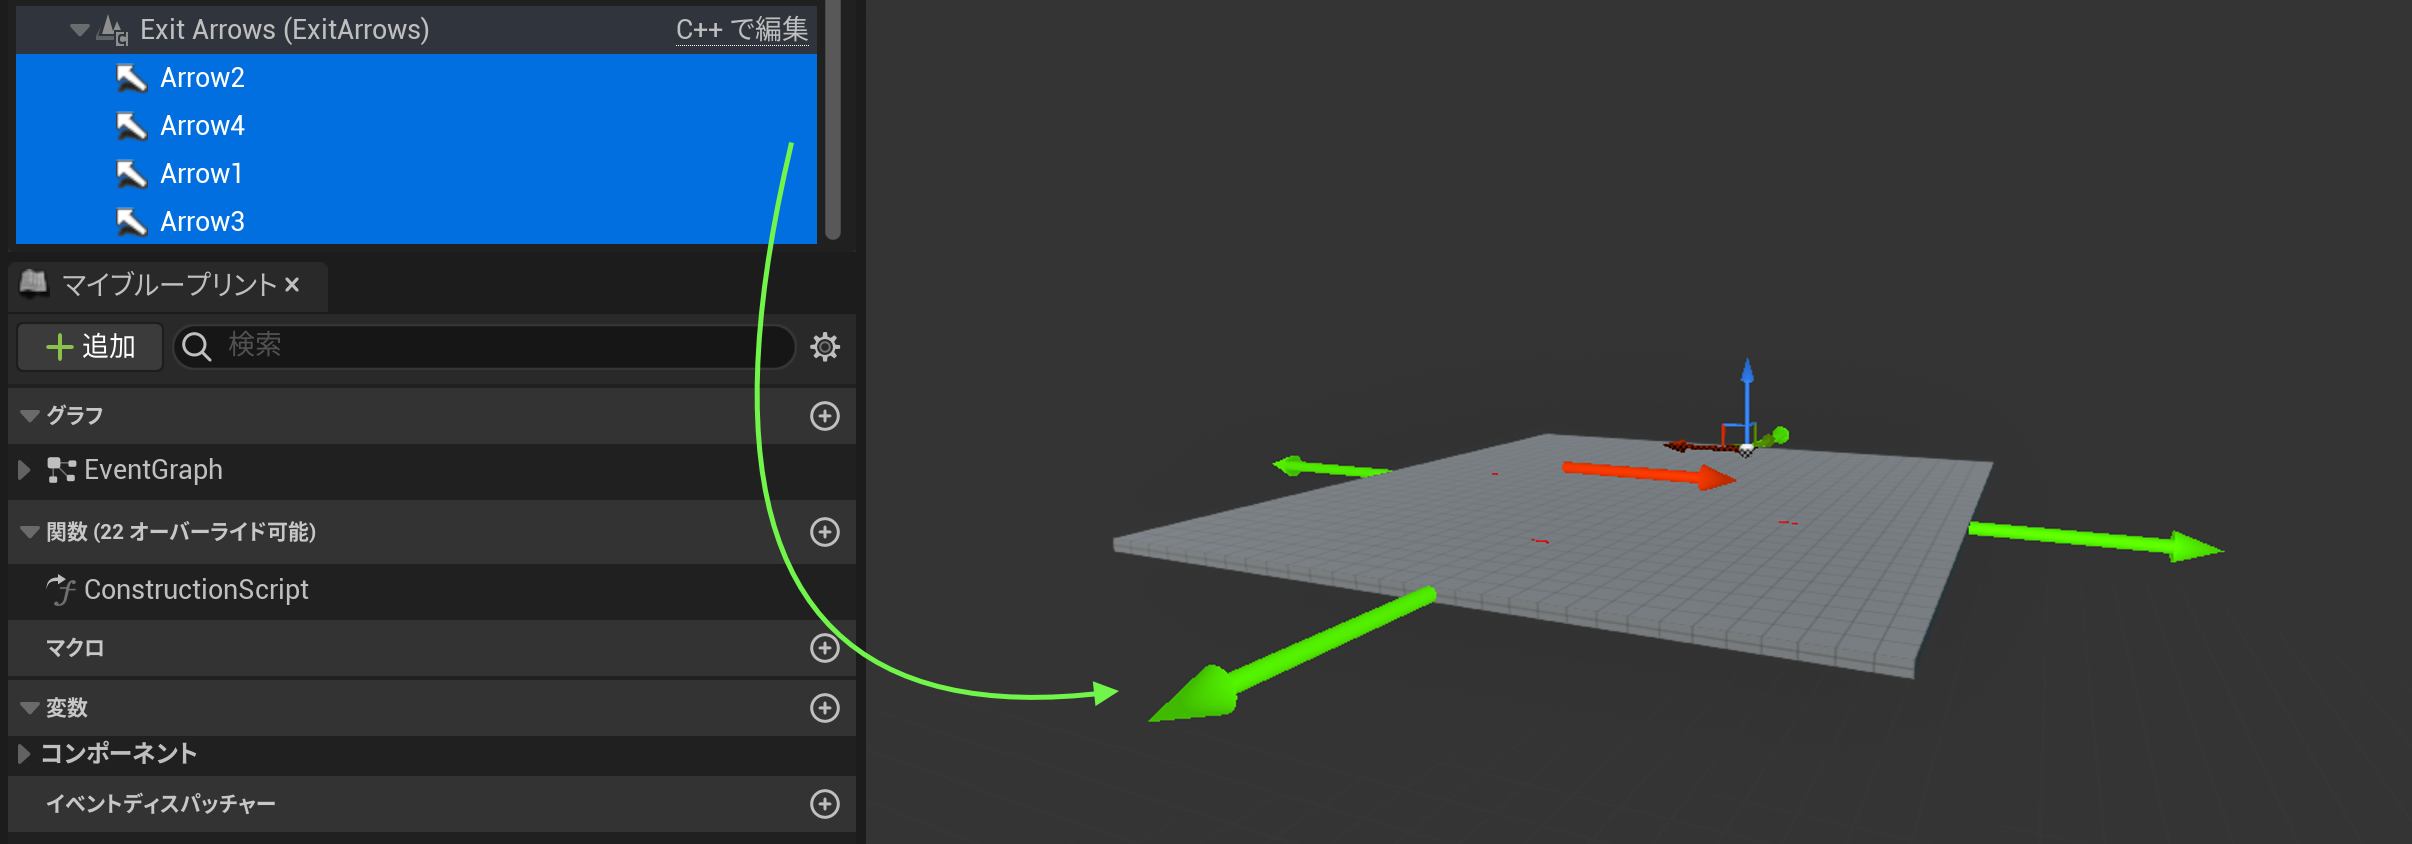
\includegraphics[scale=0.3]{IMG/ExitsPreview.png} \\
		Rooms setup\\

		\vspace{0.4cm}

		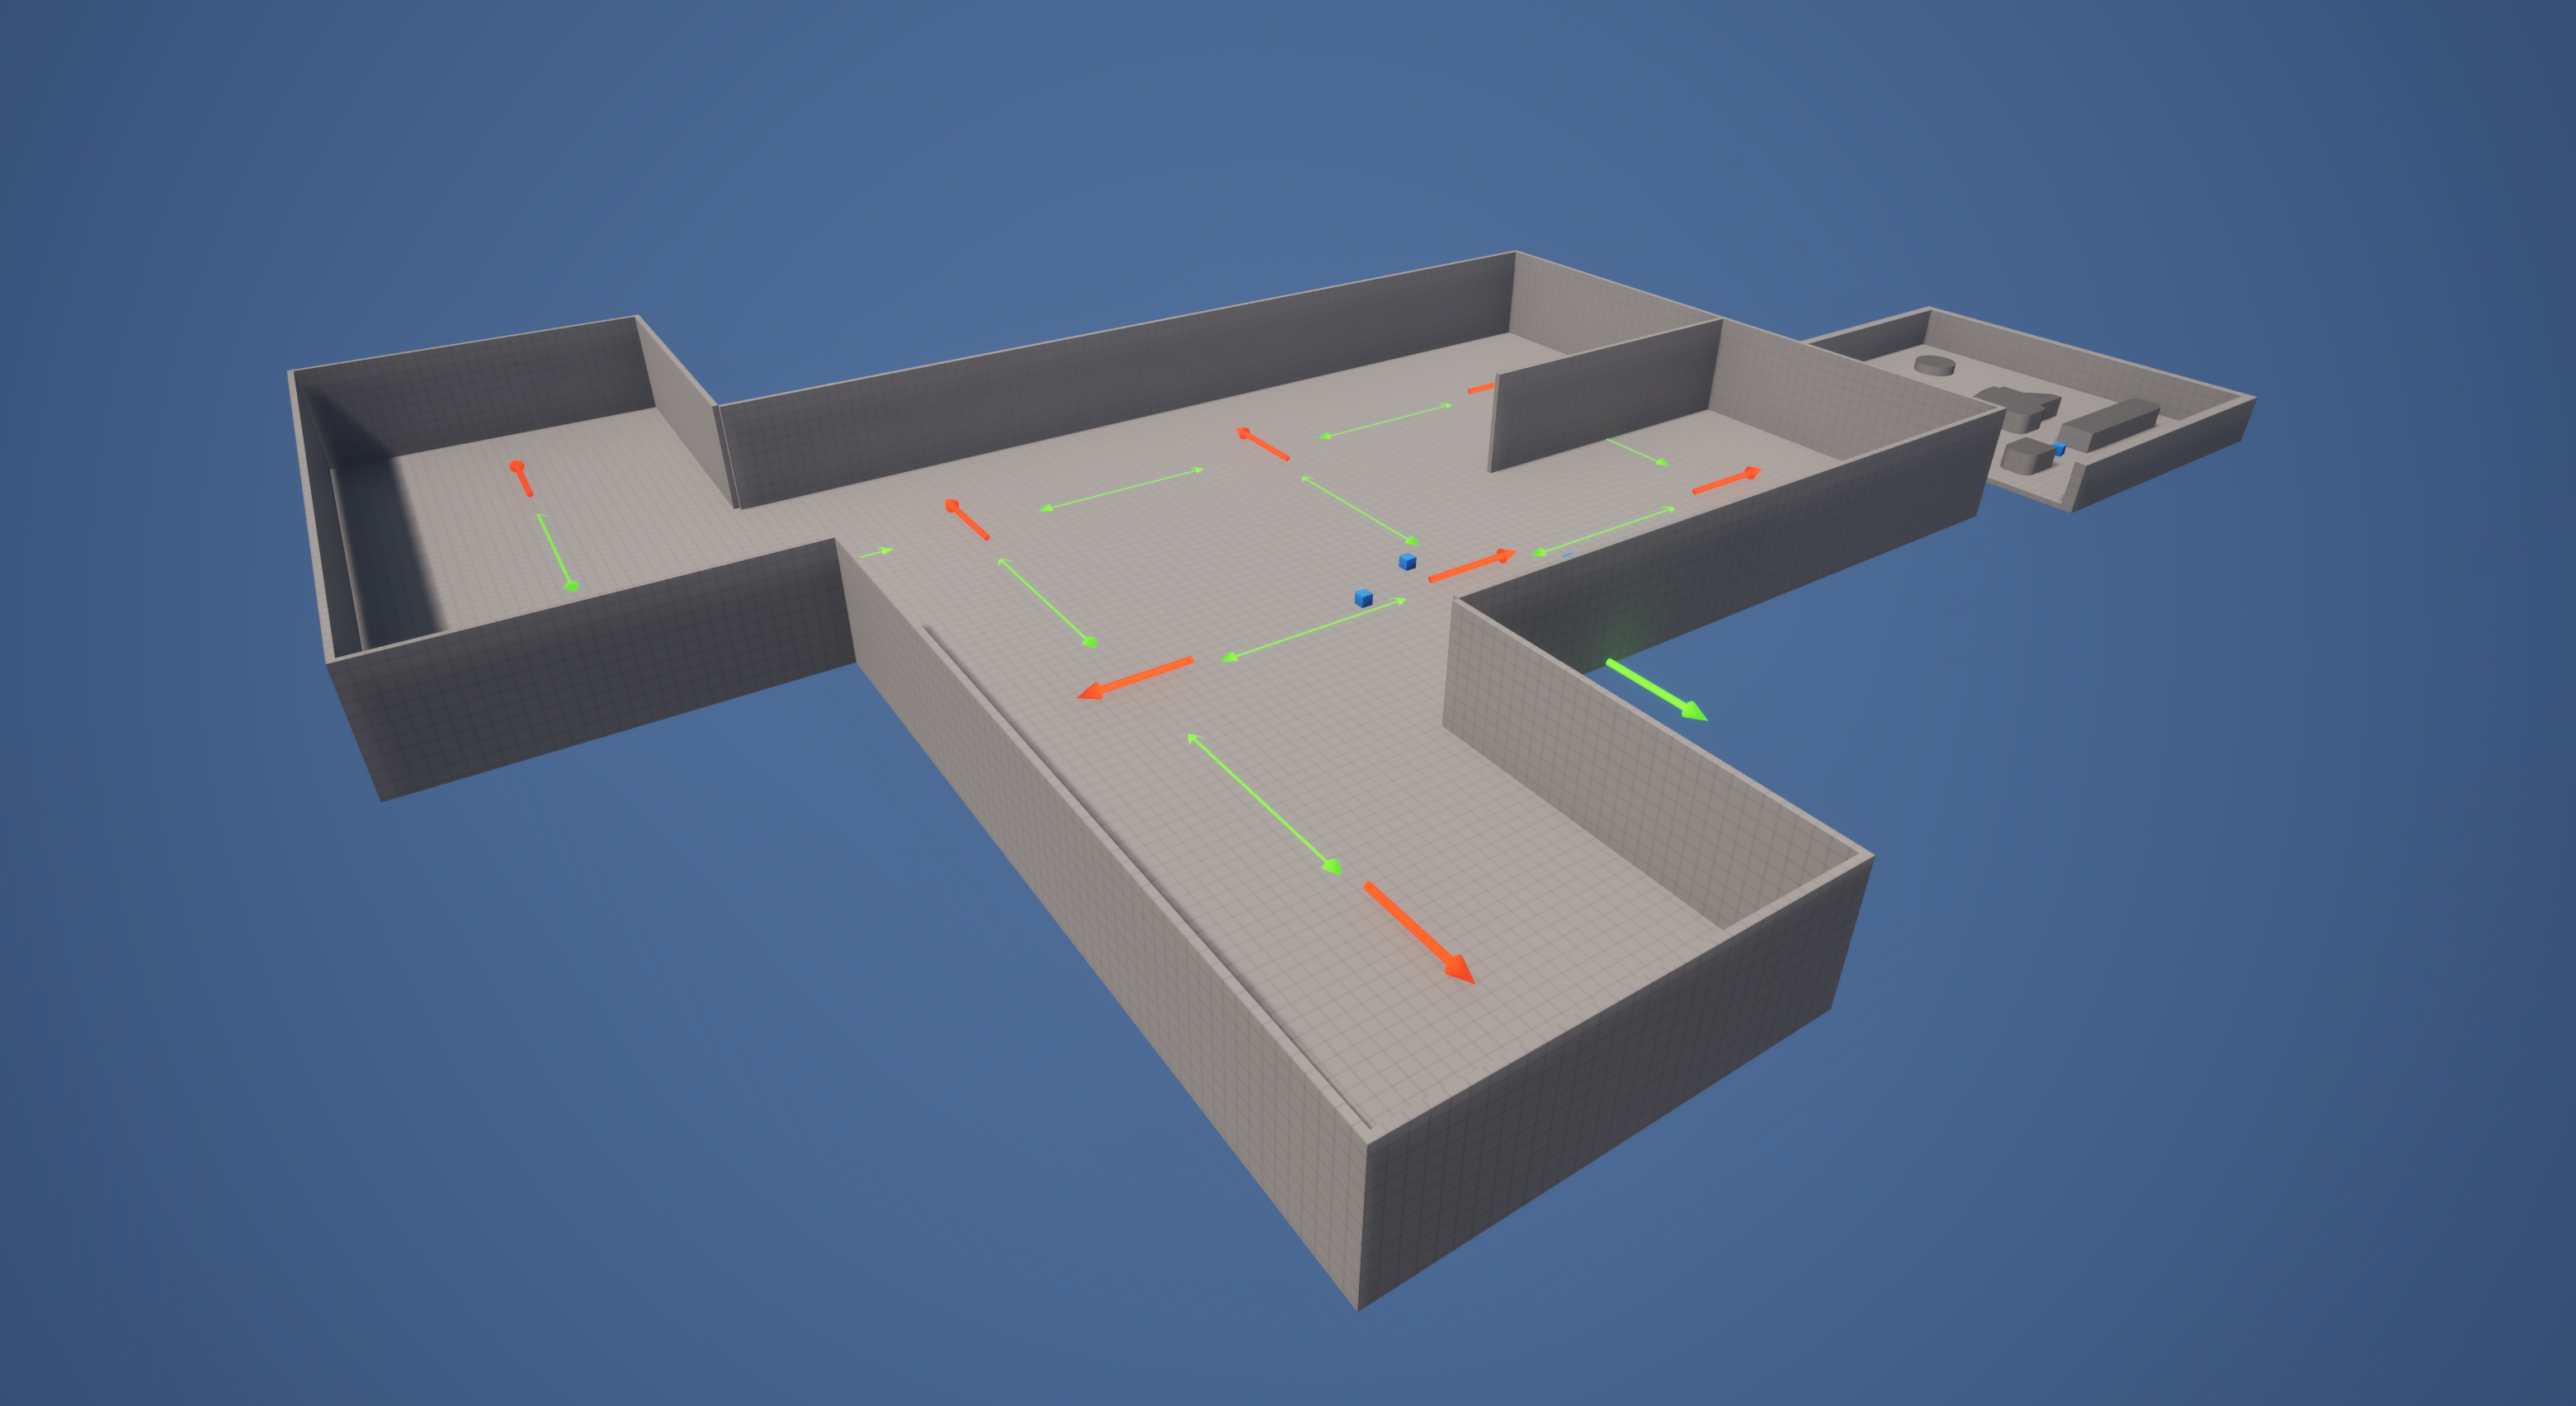
\includegraphics[scale=0.25]{IMG/ProceduralPreviewPic.png} \\
		World Generator Preview
	\end{center}

	\subsection{Collision Detection}

	But what will happen if there are no more exits available? Taking that question in consideration I created two more
	functions. The ones being reboot and delete room. The reboot function what it does is it runs the delete the room for
	each room that has been created, once all have been removed it runs a delete function for the current generator which
	awaits for all the remaining instructions to run before deleting itself. After that we run the last instruction which
	spawns a new room generator and starts the whole process again randomly generating a new world with the requirements
	given.

	But what about collision between different rooms, will it overlap? For this situation I created various functions
	that will cover collisions in different situations. This situations can be separated into two different categories.

	\textbf{General Collision:} For the general collision all we require is to get any space that it is trying to spawn and
	find if there is anything on that spot. For that the function generates a invisible tracing box which if it collides
	with anything then it tells it to look for a new spot.

	\begin{framed}
		\begin{minted}{cpp}
// Setup Box Dimensions for trace
FVector BoxDimensions = FVector(50, 50, 50);

FVector traceLocation = exitLocation.GetLocation();

// Trace box to check if collision available
FCollisionShape box = FCollisionShape::MakeBox(BoxDimensions);
exitsList[spaceIndex]->GetWorld()->SweepSingleByChannel(
    Hit,
    traceLocation,
    traceLocation,
    FQuat::Identity,
    ECC_Visibility,
    box,
    QueryParams
);

// Return true if room type has been found connected
if (Cast<AMaster_Room>(Hit.GetActor())) return true;
        \end{minted}
	\end{framed}

	\textbf{Dimension Spawn:} Based on the dimensions of the room it is trying to spawn, we require to find if there is
	sufficient space for the spot to be occupied. But to get the dimensions of said room, with the current version of
	unreal engine is not possible to pre-calculate it. For this I did a hacky solution, it was to spawn briefly the
	desired room to gets it's dimensions, save it in a transformation variable, and destroy the room. All of this is done
	really fast that we can't see the spawned room. from there on with the general collision, we pass our new calculated
	values and replace the tracing box dimensions with the new values to have precise collision testing.

	\begin{framed}
		\begin{minted}{cpp}
    // Make temporary room
AActor* roomModel = GetWorld()->SpawnActor<AMaster_Room>(
    RoomToSpawn[roomIndex],
    exitLocation.GetLocation(),
    FRotator::ZeroRotator,
    SpawnParams
);

// Setup Box Dimensions for trace
FVector BoxDimensions = FVector(roomModel->GetComponentsBoundingBox().GetExtent() - 4);
BoxDimensions.Z += 3;
roomModel->Destroy(); // Destroy tmp room after setup

FVector traceLocation = exitLocation.GetLocation() + (
    exitLocation.GetLocation() - actorLocation.GetLocation());
traceLocation.Z += BoxDimensions.Z; // Center Box Trace

// Trace box to check if collision available
FCollisionShape box = FCollisionShape::MakeBox(BoxDimensions);
        \end{minted}
	\end{framed}

	\subsection{Encapsulating World}

	In this world we are creating, we need to add some restrictions for the entities. These restrictions will help prevent
	the entities of walking off bounds and falling to the emptiness. The main focus for this project isn't for them to learn
	where they can fall off from, but how to react to the interaction between various entities. For this preventions, I
	decided to encapsulate the exits which have been left empty at the end of the generation with walls.

	For the closing of the walls we might want to prevent them from spawning in places which connect to different rooms.
	If we did not do this then it will not be different from making a maze. Lets mention how I differentiate between
	generating a world, and a maze. A maze is generally restrictive. The movement is constrained by paths bordered by
	walls which is generally defined as corridors. While a world in this case we see it less restrictive which has is
	composed by corridors and open spaces.

	To prevent walls for being created everywhere, small trace boxes are created. This trace boxes are made just in order
	to find out if there is any rooms connected to the desired spot that the wall wants to be allocated. If there is a
	connected room than we remove from the opened exit list and move on to the next exit to close. If the desired room
	to spawn can not be placed in any of the exits, this is removed from the possible rooms to spawn and moves on to the
	next room until no more exits and rooms are available.

	\begin{center}
		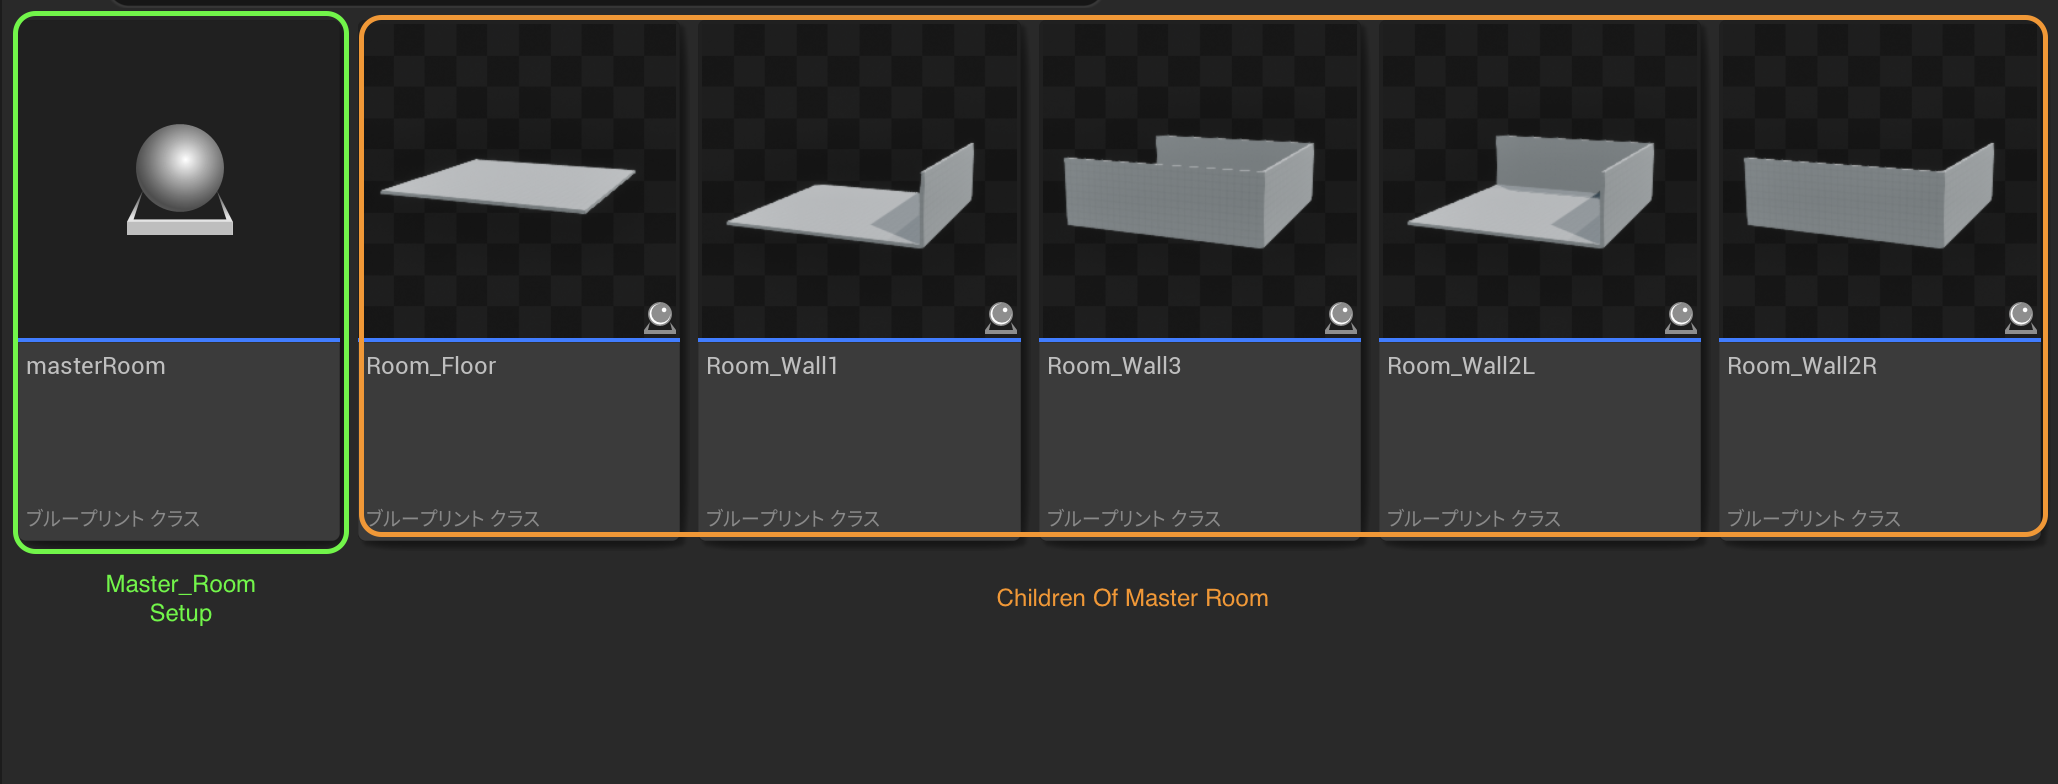
\includegraphics[scale=0.4]{IMG/MasterRoomChildrenPreview.png} \\

		Creation of Rooms
	\end{center}

	\subsection{Seed}

	At some point I realized that we might want to keep the entities in a specific room for a period of time. For this
	I had decided to add a seed option\footnote{More information can be found at https://github.com/AndreM222/Procedural-Generator/blob/main/docs/setup.md}
	. When a seed is used then depending on the number it will generate a room which no matter how many reloads it goes through,
	it always stays the same. But the problem of using a seed is there will be an opportunity for the desired total rooms to
	be spawned to not be able to take place. This is phenomenon could happen by the rooms spawning in a specific path, which at
	some point could end up eating its own tail and not having any other available exit. For this case, I told the generator to
	skip the loop of making new generators till one goes accordingly with the requirements. The reason of this is to prevent a
	infinite loop from happening.

	\begin{center}
		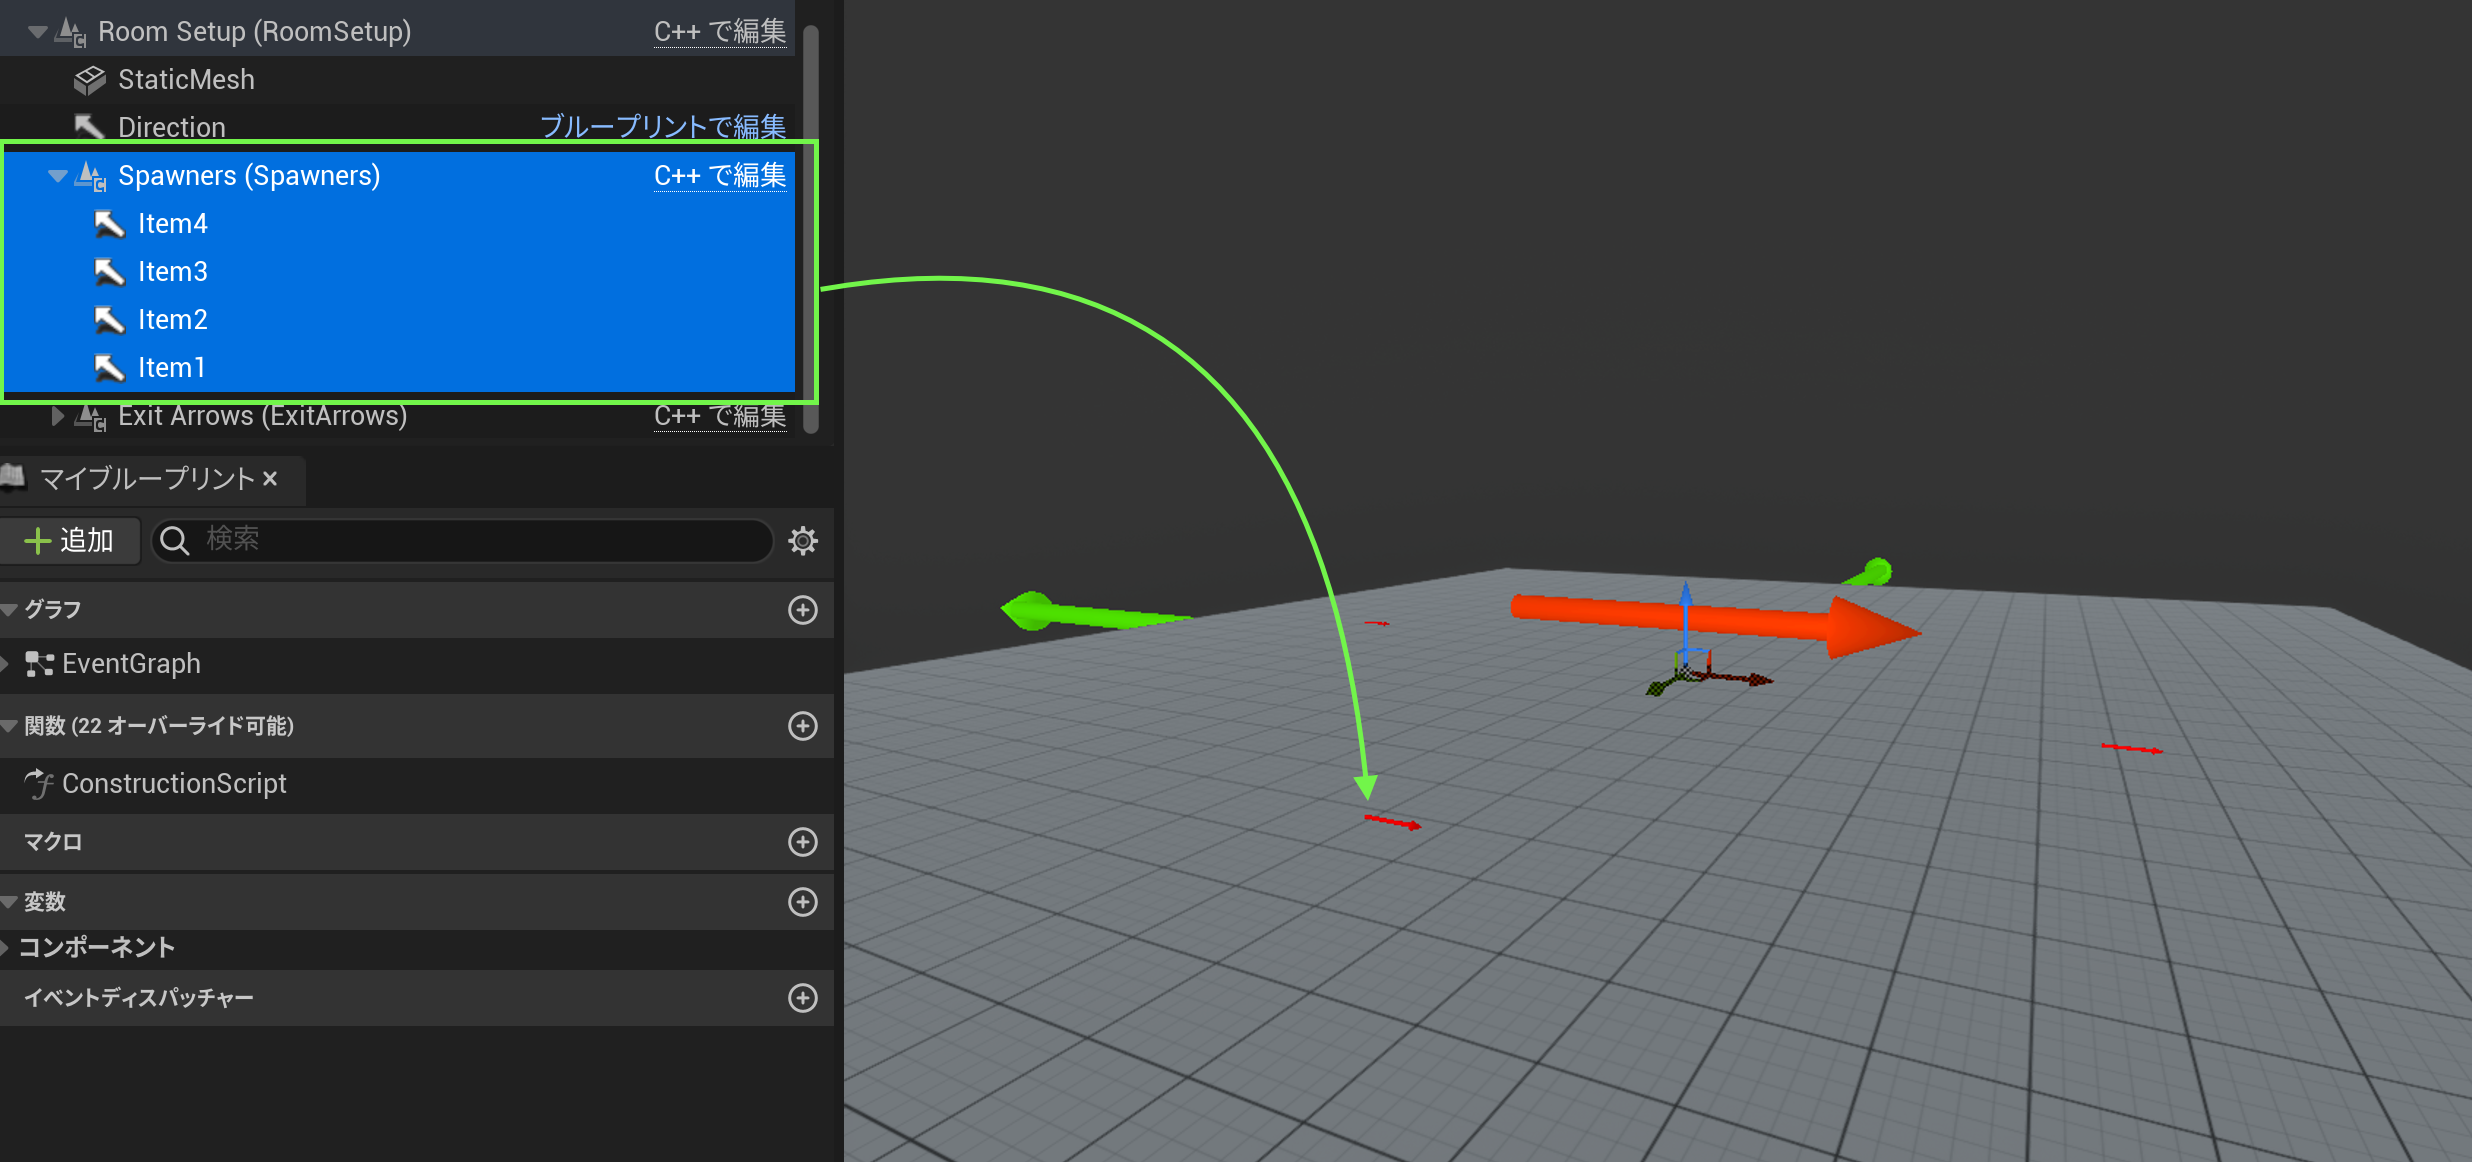
\includegraphics[scale=0.3]{IMG/SpawnPointsPreview.png} \\
		Props Spawner \\

		\vspace{0.4cm}
		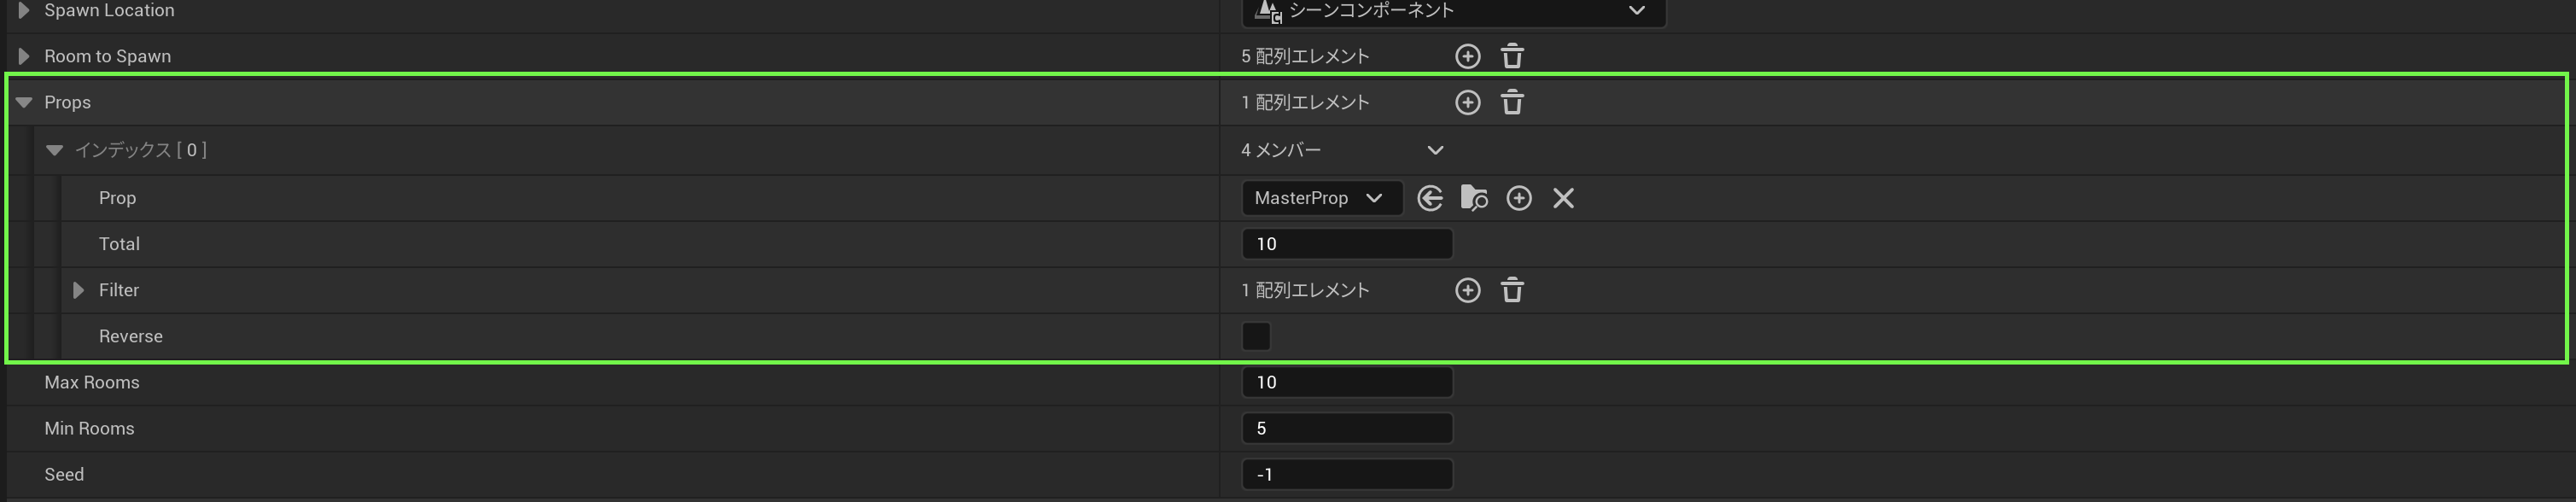
\includegraphics[scale=0.3]{IMG/PropsPreview.png} \\
		Props settings

	\end{center}

	\subsection{Props and Spawners}

	To add spawners for the entities and as well adding obstacles, I implemented a spawning function which spawns randomly
	with filter capabilities actors we desire to spawn throughout the rooms. This look for the spawning arrows in the spawners
	folder.

	\section{Character Setup}

	For the 3D model and the animations I am using the assets of a pack called \citetitle{AdvanceLocomotionSystemV4} \parencite{AdvanceLocomotionSystemV4}. This
	Pack contains a whole of useful animations and some simple models that I could benefit from to focus on the development
	of the actions and thinking of the characters.

	This pack also comes with a setup for movement but it was fully done in blueprints which is not easily accessible
	with C++, so for this situation I made my own logic regarding the interaction the entities\footnote{Code can be found at https://github.com/AndreM222/AI-Entities} do in the 3D space.
	The behaviors included in the project where all done using blueprints. This is one of the perks of Unreal Engine,
	but an issue arises. At the moment is not possible to interact from C++ to blueprints, but it can be done backwards.
	So currently I made my own version of locomotion for realistic movement but with the animations from the package.

	\begin{center}
		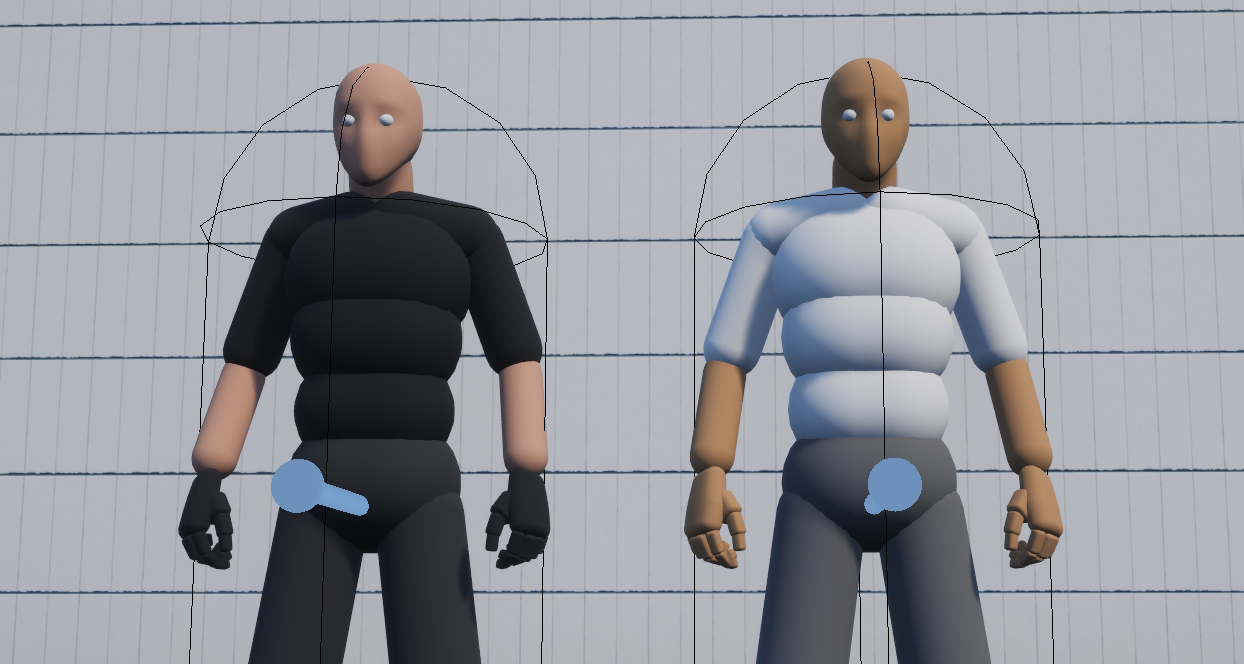
\includegraphics[scale=0.6]{IMG/Teams-Picture-Preview.png} \\

		Character Setup
	\end{center}

	\subsection{States}

	States are the different stances in which the entities can change depending on their interaction. For applying more
	human-like interactions in the real world. Interactions could have been done without animations but if we want to
	take into consideration delays in reaction and ease of showcase, I decided to use the asset pack animations to make
	this possible. The following are the available states made.

	\begin{itemize}
		\item \textbf{Used:} Is currently being used for some kind of interaction.
		\item \textbf{Planned:} Is ready to be used but has not combined it with the logic to activate it.
	\end{itemize}

	\begin{center}
		\begin{tabular}{|l|l|l|}
			\hline
			Stance     & Description                                                    & State   \\
			\hline
			Default    & Is a stance which invokes neutrality and peace                 & Planned \\
			\hline
			Masculine  & Is ready for combat or try to show power                       & Used    \\
			\hline
			Feminine   & Is more graceful and noble stance                              & Planned \\
			\hline
			Injured    & Shows the low amount of health the entities have               & Used    \\
			\hline
			HandsTied  & This will showcase the when restriction is present in entities & Planned \\
			\hline
			Rifle      & Holding a riffle                                               & Planned \\
			\hline
			Pistol 1H  & Holding a pistol with 1 hand                                   & Planned \\
			\hline
			Pistol 2H  & Holding a pistol with 2 hands                                  & Planned \\
			\hline
			Bow        & Holding a bow                                                  & Planned \\
			\hline
			Torch      & Holding a torch for illumination                               & Planned \\
			\hline
			Binoculars & Holding binoculars to see from far away                        & Planned \\
			\hline
			Box        & Carrying boxes                                                 & Planned \\
			\hline
			Barrel     & Carrying a barrel                                              & Planned \\
			\hline
			Reach      & Is a stance for reaching towards the target to touch for range & Planned \\
			\hline
		\end{tabular}
	\end{center}

	\section{Actions}

	Actions is the different capabilities the entities have to interact with the world. This adds more complexity
	and variety to the thinking of the entities.

	\begin{center}
		\begin{tabular}{|l|l|l|}
			\hline
			Action & Description               & State   \\
			\hline
			Run    & High speed movement       & Used    \\
			\hline
			Sprint & Medium Speed Movement     & Used    \\
			\hline
			Walk   & Slow speed movement       & Used    \\
			\hline
			Crouch & Crouching in small spaces & Used    \\
			\hline
			Climb  & Climb walls               & Used    \\
			\hline
			Grab   & Grab a prop               & Planned \\
			\hline
			Drop   & Drop item holding         & Planned \\
			\hline
			Jump   & Jumping                   & Used    \\
			\hline
			Touch  & Touch the target          & Used    \\
			\hline
		\end{tabular}
	\end{center}

	\begin{center}
		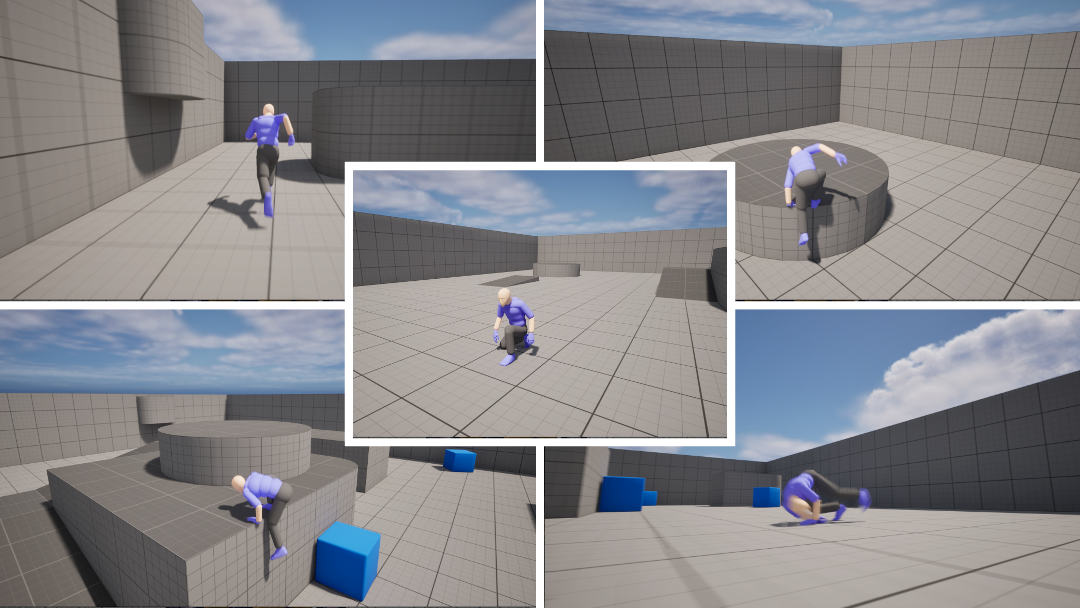
\includegraphics[scale=0.4]{IMG/ActionPreview.png} \\
		Previews Of Actions
	\end{center}

	\section{Decision Making Through Genomes}

	I have started the development of the character intelligence with the use of genomes, but it is still missing
	a variety of functions for them to make rational choices through generations of data being provided from parents.

	This application was successful to run in simple tasks like the entities having the need to go to specific areas
	of the map. But tag is a more complex task which will require more data and capabilities for the entities.

	\subsection{Genetic Algorithm}

    For more detail on how this works is through the use of genetic alogithm \parencite{GeneticAlgorithm}. Which this means is the use of evolition.
	As to decision making, we could let one entity just try to wire its own brain with something called a mutation. But
	there will be a limit to how much it can grow, or find better ways of solving a problem. As you all know when it comes
	to self development there are internal and external factors which help us grow. Internal are seen as things we
	experienced and we use to make decisions, but as for external are does who teach us of their experience. This
	factor makes not only grow which thats what internal does, but grow in the most efficient way.

    \begin{center}
        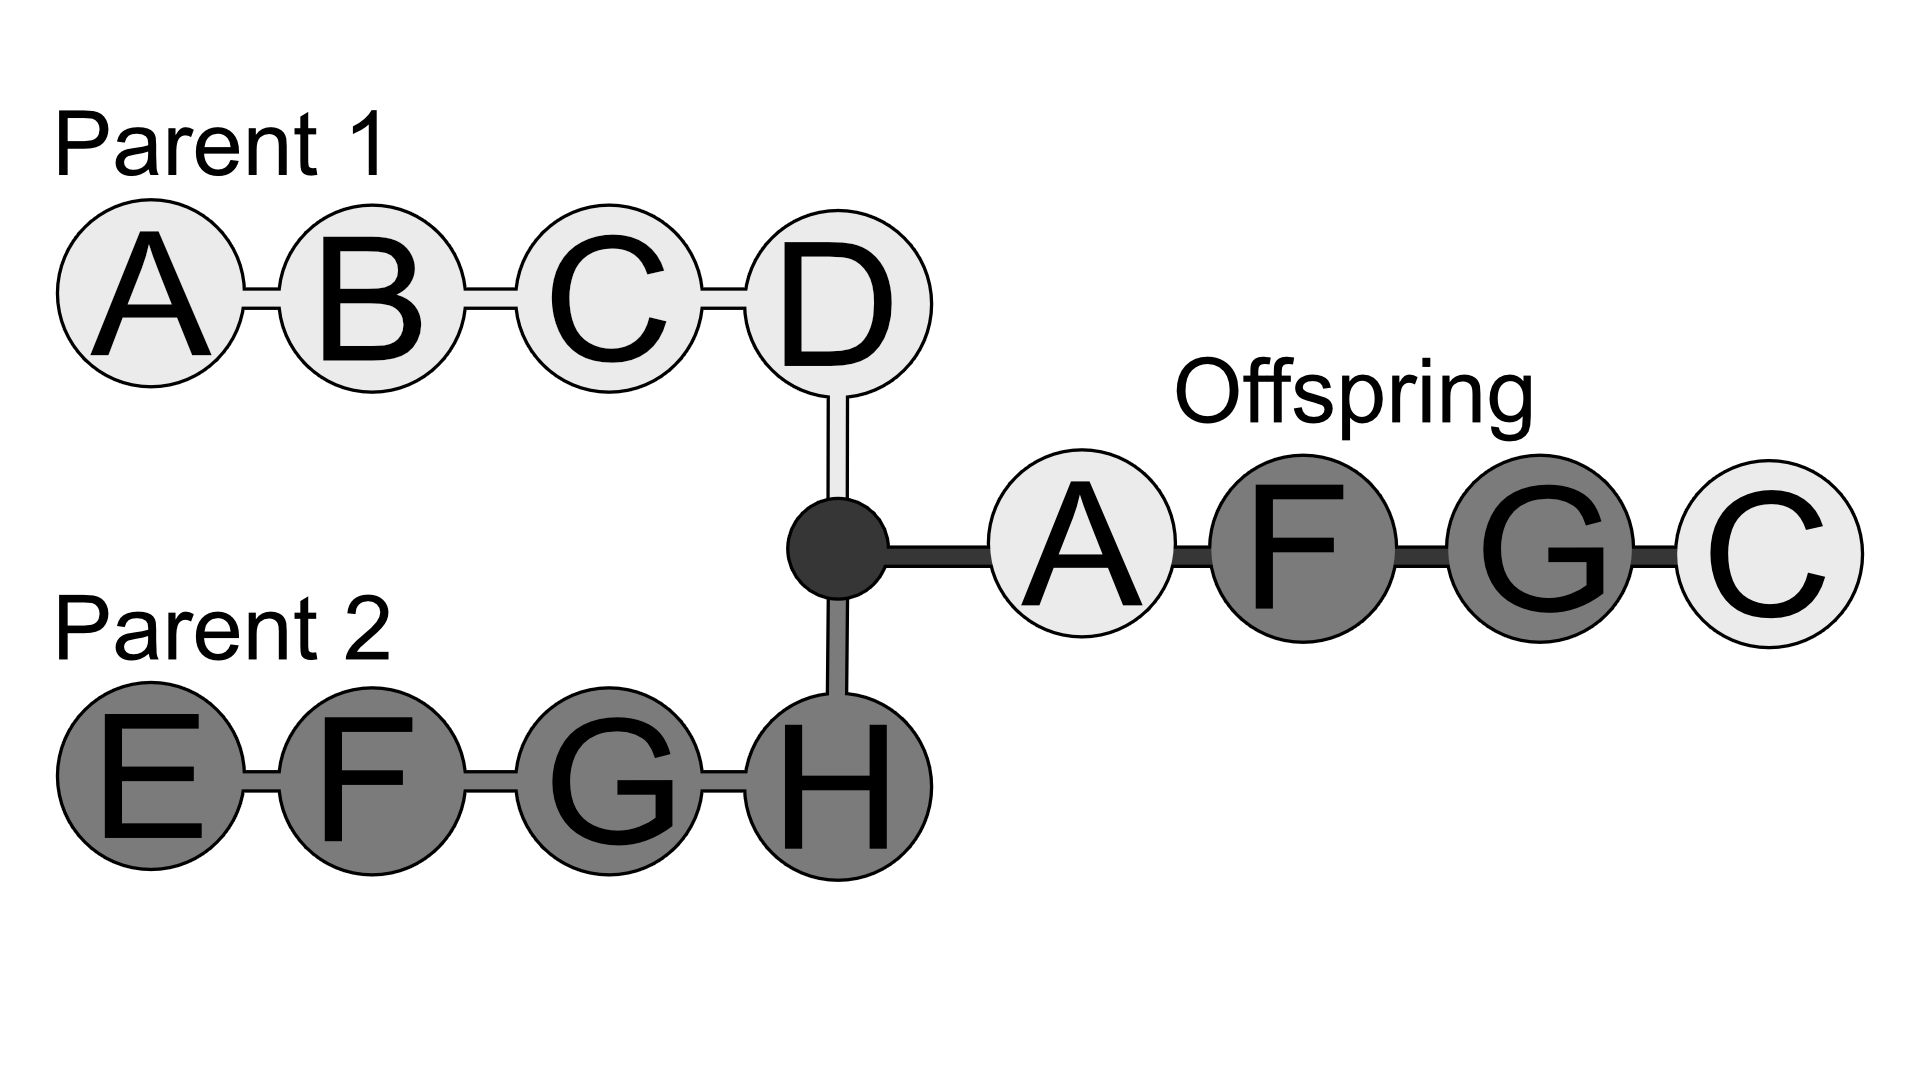
\includegraphics[scale=0.15]{IMG/GeneticAlgorithm.png} \\
        Genetic Algorithm
    \end{center}

	\subsection{NEAT Algorithm}

    NEAT Algorithm \parencite{NeatAlgorithm} utilizes the genetic algorithm, but it puts the idea of genomes into action to develop their brains.
	By having the senses, actions, and the internal neurons. These neurons wire up as augmented topologies which
	means that their brain evolves as it desires. But as to have some control over we set up a max limit of neurons.

	The algorithm will grab two parents and combine them by using pheromones dictated by their likeness, which in this
	case is defined as how well they solve their task. All of these neurons can combine with each other and themselves.
	But for some cleanup, we set up a function that detects if some connection is not doing anything by itself and deletes it.

	If an entity has too many senses it can get overwhelmed and not do their actions correctly, but if it has too little
	then it won't find the best way of solving a problem.

    \begin{center}
        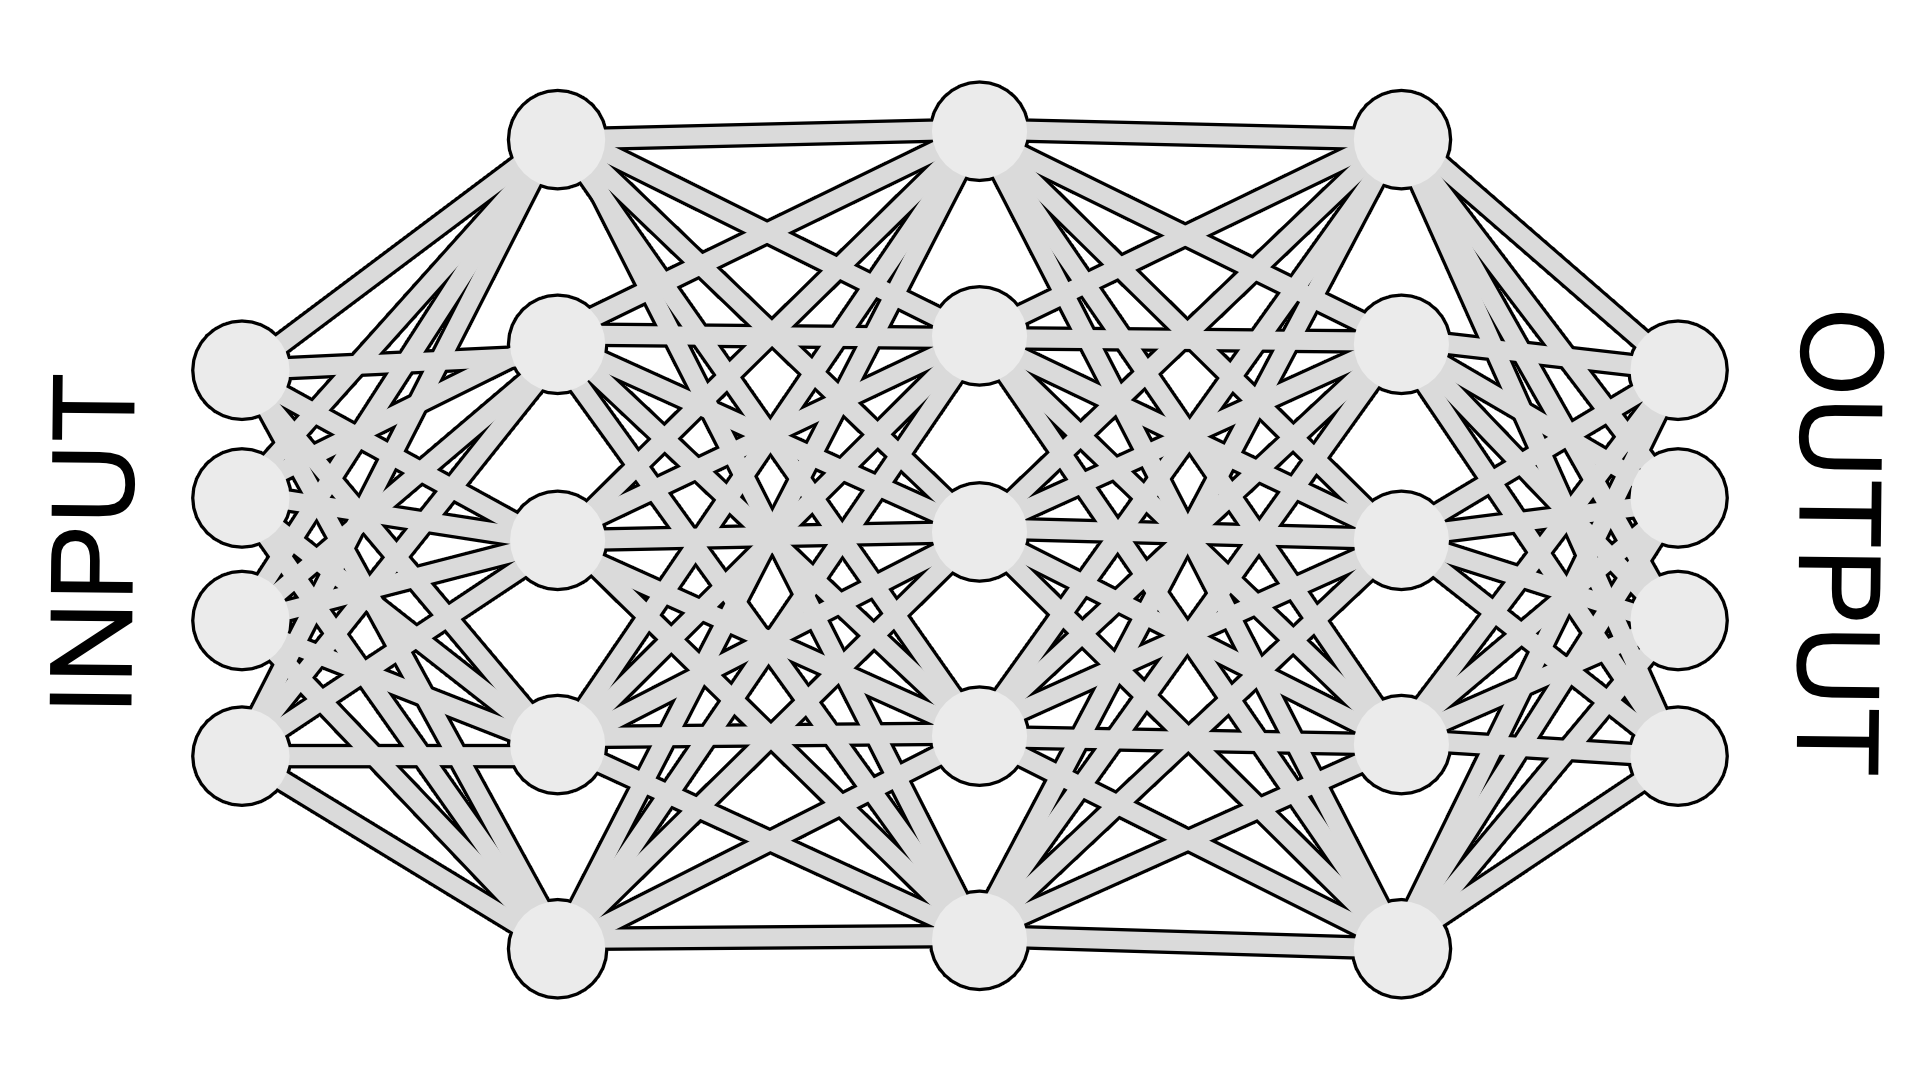
\includegraphics[scale=0.15]{IMG/NeatAlgorithm.png} \\
        NEAT Algorithm
    \end{center}

	\subsection{Senses}

	For these entities, I started developing senses like humans have. By senses, I mean by sense of hearing, sense of sight, etc.
	But for this project we will limit this to the following.

	\begin{center}
		\begin{tabular}{|l|l|l|}
			\hline
			Type of Sense & Description                                                              & Status         \\
			\hline
			Space         & This sense will give the entities the ability to know where they are.    & Being Used     \\
			\hline
			Touch         & It will be used to obtain data of their interaction to decide if they    & In Development \\
			              & like or dislike.                                                         &                \\
			\hline
			Sight         & For the entities to know what is in front of them and decide what to do. & Being Used     \\
			\hline
		\end{tabular}
	\end{center}

	But every input has subdivisions which create extra complexity. For example in order to get sight we need to
	get the distance of actors, distance of wall, quantity of population, and so on. For this, a variety of tracings
	are used in order to calculate distance, quantity, whats in front, etc.

	\begin{center}
		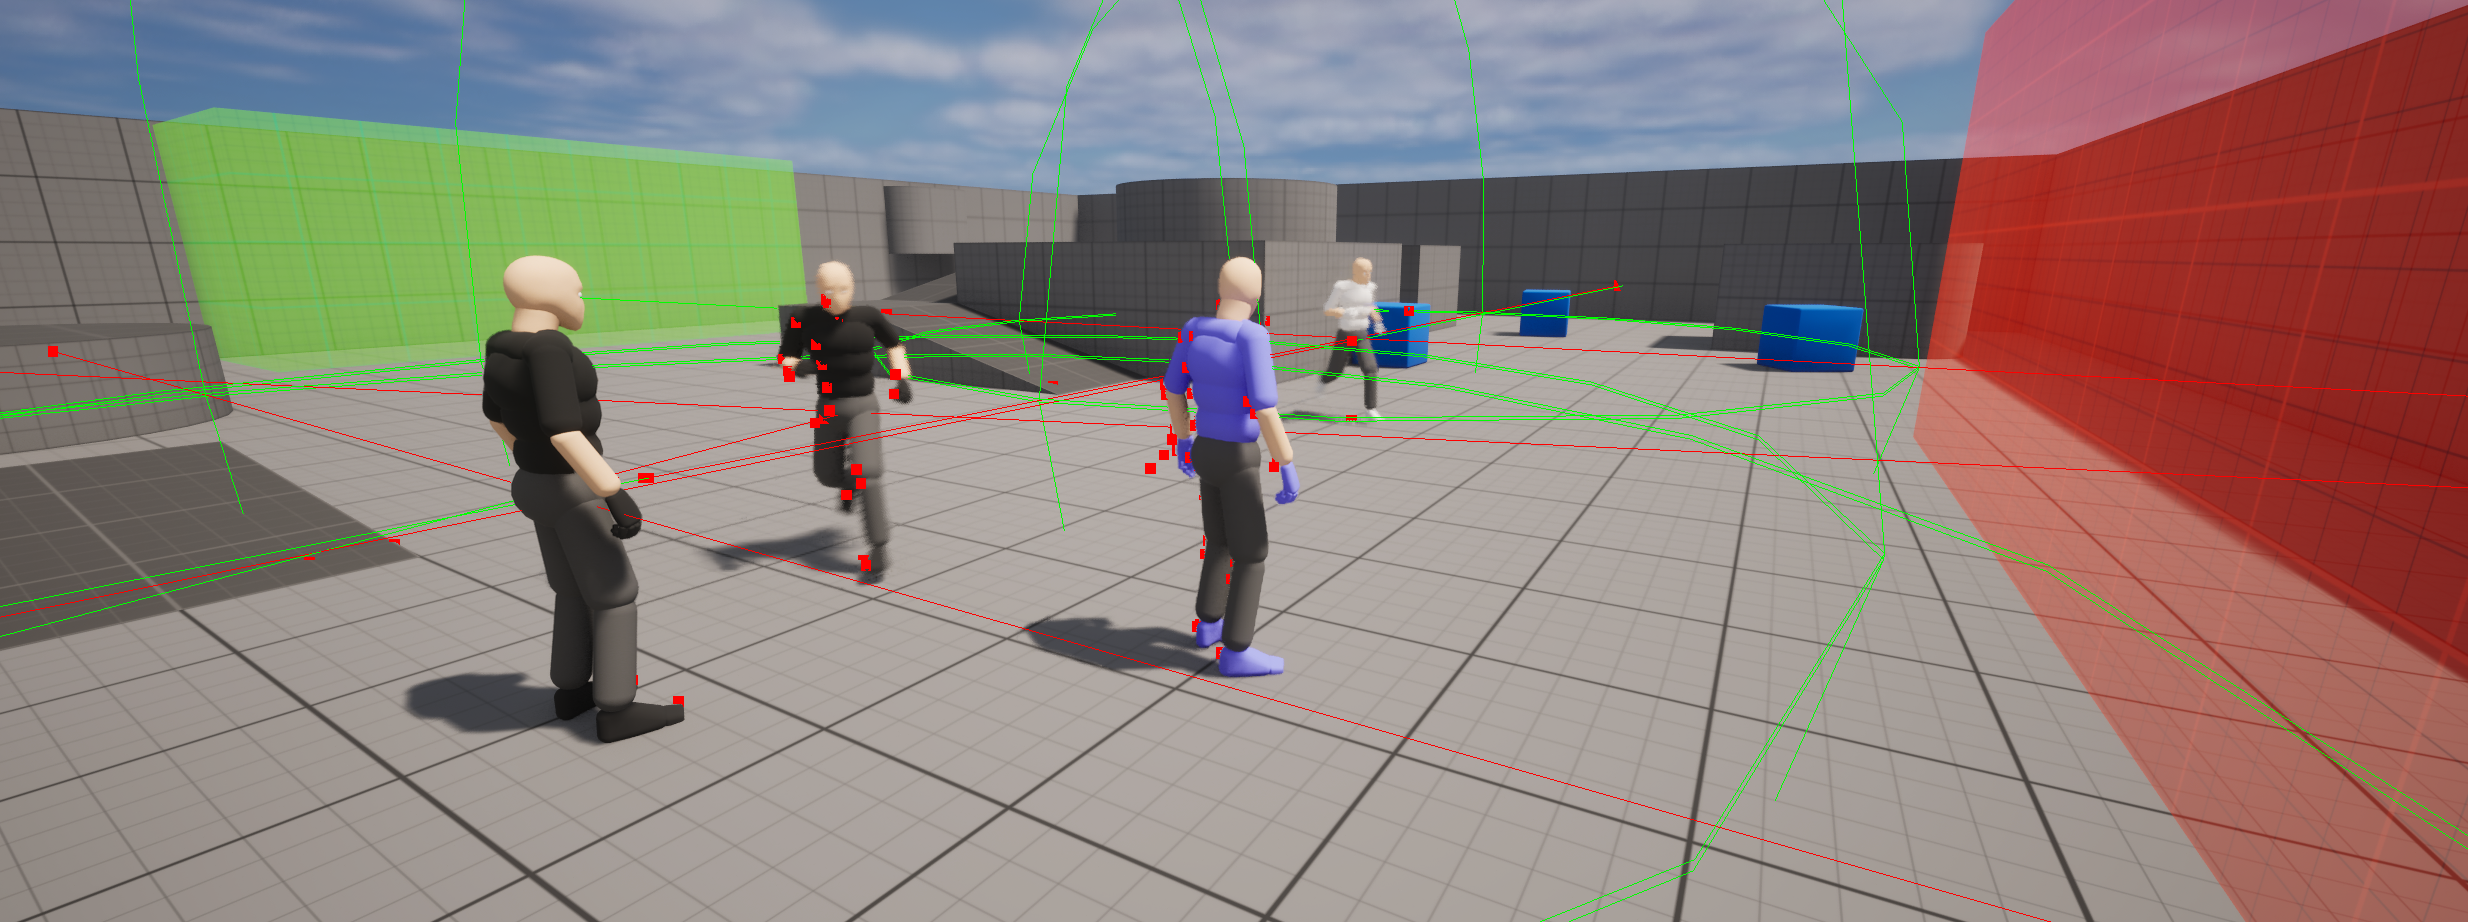
\includegraphics[scale=0.35]{IMG/TracingSense.png} \\
		Previews Of Senses
	\end{center}

	The initial behavior had only running, jumping, and climbing as actions. For senses, we detected population
	density and distance as well as a very minimal setup of boundary distance. The characters started only going
	in circles and not doing anything special. So we added more senses and actions like ledge detection, current location
	based on boundaries, and normalized values, we increased their thinking process and they started navigating more, some
	of them not doing anything, and some jumping if either a wall was detected nearby or the contrary. This was fascinating
	to see as how they started developing more the more they could sense and do.

    \section{All In One}

    Since this project scale is quite large and as well many assets could be used for testing which wont be needed at the
    final product, I separated all the components in different repositories. But this will mean that there should
    be a mergin at some point. Unreal Engine is not as easy to work when it comes to mergin different projects
    into one as other tools, so I required to make a automated merger using a cmakelist
    \footnote{For merged project go to https://github.com/AndreM222/Tag-AI-Sandbox}.

    This project will handle the UI and the communication between all of the components made without affecting
    the original scripts. This makes it secure to prevent breaking code by isolating it in different repositories.

    \subsection{Why CMake}

    I thought originally to make a bash file to run the merging between the projects, but this would limit the
    setup on specific operating systems. CMake, even though a installation is required, the process of running
    works cross-platform making it an ideal choice.

    \subsection{How To Add}

    To make the setup easier, I decided to use a json file to list the projects desired to merge as well
    with a filtering option. This merger takes care of removing the non-important files like the build and
    main script of the projects and replaces all of the APIs with the current project one.

	\section{Evaluation}

	\subsection{Path}
	The entities seem to end up following a pattern of going to specific directions until is able to either touch
	its target, or avoid it. But there seems to be a constant improvement over time of their behavior and adaptation in
	different environments.

	I tried running it through the same requirements as the \citetitle{ProgrammedSomeCreatures} \parencite{ProgrammedSomeCreatures}
	to test out what will happen with a more basic mission like going to specific areas of the map. As I run them,
	they ended up reacting the same. This might be because a game of tag requires to have senses like sight, touch,
	and sense of space. To make more rational decisions.

	\subsection{Obstacles}
	As not many test have been run, for now the entities seem to walk towards the wall in certain angles until is able to cross
	to the other side if needed.

	More testing will be required to see how their behavior improves over time.

	\section{What Comes Next}

	I will continue developing the structure for their decision making and move the project to the super computer to start
	obtaining data while I keep implementing features.
	I also need to develop a UI which can give me data from the occurrences and as well take screenshots every generations.
	While the entities are running in the background I will be working on the extra behaviors to implement them.

	To improve the decision making of the entities I will start incorporating some senses to them. This will improve
	their decision making by being able to choose location based on where they where, touch, or saw. As well what
	they find as interesting, dangerous, or non-important.

	The entities behavior is still primitive and require further development to see their improvement in their behavior.
	Further iterations are required to see how they interact more with their environments and if they successfully are able to
	learn how to catch or escape from the target.

\end{Form}

\printbibliography[heading=bibintoc]

\end{document}
